\section{Szymon Szkarłat}
\label{sec:szymon_szkarlat}

\centering{Pies - najlepszy przyjaciel człowieka! (zobacz Zdjecie~\ref{fig:dog}).}

\begin{figure}[htbp]
    \centering
    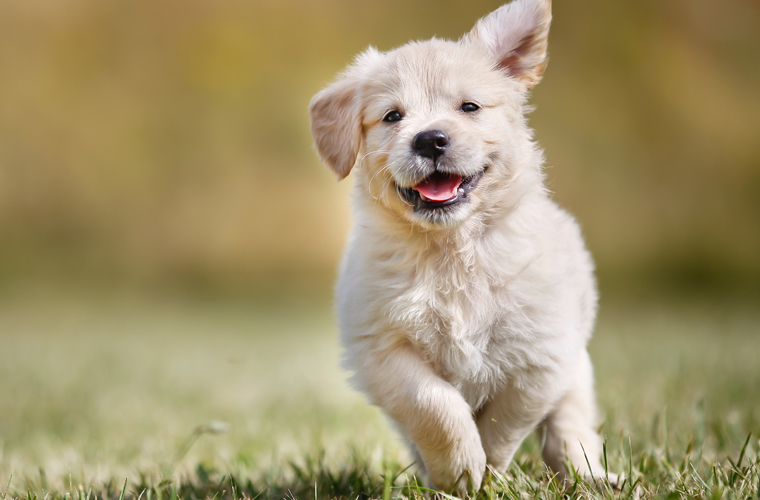
\includegraphics[width=0.9\textwidth]{pictures/pies.jpg}
    \caption{Wesoły piesek.}
    \label{fig:dog}
\end{figure}

Tabela~\ref{tab:tabela_ucl} UEFA Champions League 22/23 - group G

\begin{table}[htbp]
\centering
\begin{tabular}{||c c c c||} 
 \hline
 Miejsce & Drużyna & Punkty & Bilans bramkowy \\ [0.5ex] 
 \hline\hline
 1. & Manchester City & 14 & 14:2 \\ 
 \hline
 2. & Borussia Dortmund & 9 & 10:5 \\
 \hline
 3. & Sevilla & 5 & 6:12 \\
 \hline
 4. & FC Kopenhaga & 3 & 1:12 \\
 \hline
\end{tabular}
\label{tab:tabela_ucl}
\caption{Wyniki fazy grupowej Ligi Mistrzów sezonu 2022/23}
\end{table}

{\Large Proste wyrażenie matematyczne ;)
 \[(a-b)^3=a^3 - 3a^2b + 3ab^2 - b^3\]}

\section*{Polecenia sieciowe w kosoli CMD:}
\begin{enumerate}
  \item \textbf{ipconfig} - wyświetla podstawowa konfiguracje karty sieciowej komputera.
  \item \textbf{ipconfig /all} - wyświetla rozbudowana konfiguracje karty sieciowej, pokazujac miedzy innymi \underline{adres fizyczny} (MAC).
  \item \textbf{ping} - służy do sprawdzenia komunikacji pomiedzy naszym urzadzeniem sieciowym a odległym hostem.
\end{enumerate}

Lista rzeczy do zrobienia:
\begin{itemize}
  \item Pojść do lekarza
  \item Posprzatać pokój 
  \item Umyć okna
  \item Wyjść z psem na spacer
  \item Zrobić zakupy
  \item Pójść spać
\end{itemize}

\setlength{\parindent}{20pt}
\section*{Pies - przyjaciel czlowieka!}
\textbf{Psy}, potrafia skutecznie poprawić nam \textbf{nastrój}. Dzieje się tak dlatego, że podczas kontaktu z nimi nasz organizm wydziela endorfiny tzw. \textit{hormony szcześcia}. Im jest ich \textbf{wiecej}, tym \textbf{niższym} poziom odczuwanego stresu.

\textbf{Psy} swietnie wyczuwaja \underline{ludzkie nastroje}. Gdy jest Ci smutno, zwierzak najczesciej odwzajemnia to i nie przeszkadza zachecaniem do zabawy.  

\textbf{Z kolei}, gdy Ty tryskasz \underline{radościa} – on rowniez. Czyz to \textbf{nie powod}, by mówić o psie: \textbf{\textit{najlepszy przyjaciel człowieka?}}